\documentclass[11pt,a4paper]{jsarticle}
%
\usepackage{amsmath,amssymb}
\usepackage{bm}
\usepackage{graphicx}
\usepackage{ascmac}
%
\setlength{\textwidth}{\fullwidth}
\setlength{\textheight}{40\baselineskip}
\addtolength{\textheight}{\topskip}
\setlength{\voffset}{-0.2in}
\setlength{\topmargin}{0pt}
\setlength{\headheight}{0pt}
\setlength{\headsep}{0pt}
%
\newcommand{\divergence}{\mathrm{div}\,}  %ダイバージェンス
\newcommand{\grad}{\mathrm{grad}\,}  %グラディエント
\newcommand{\rot}{\mathrm{rot}\,}  %ローテーション
%
\title{リンゴについて}
\author{早川悠介}
\date{\today}
\begin{document}
\maketitle
%
%
\section{リンゴとApple}
iPadに描いたリンゴはAppleのリンゴとは違う。
まず第一に、形状が違う(図\ref{fig:apple})。

\begin{figure}[htbp]
\begin{center}
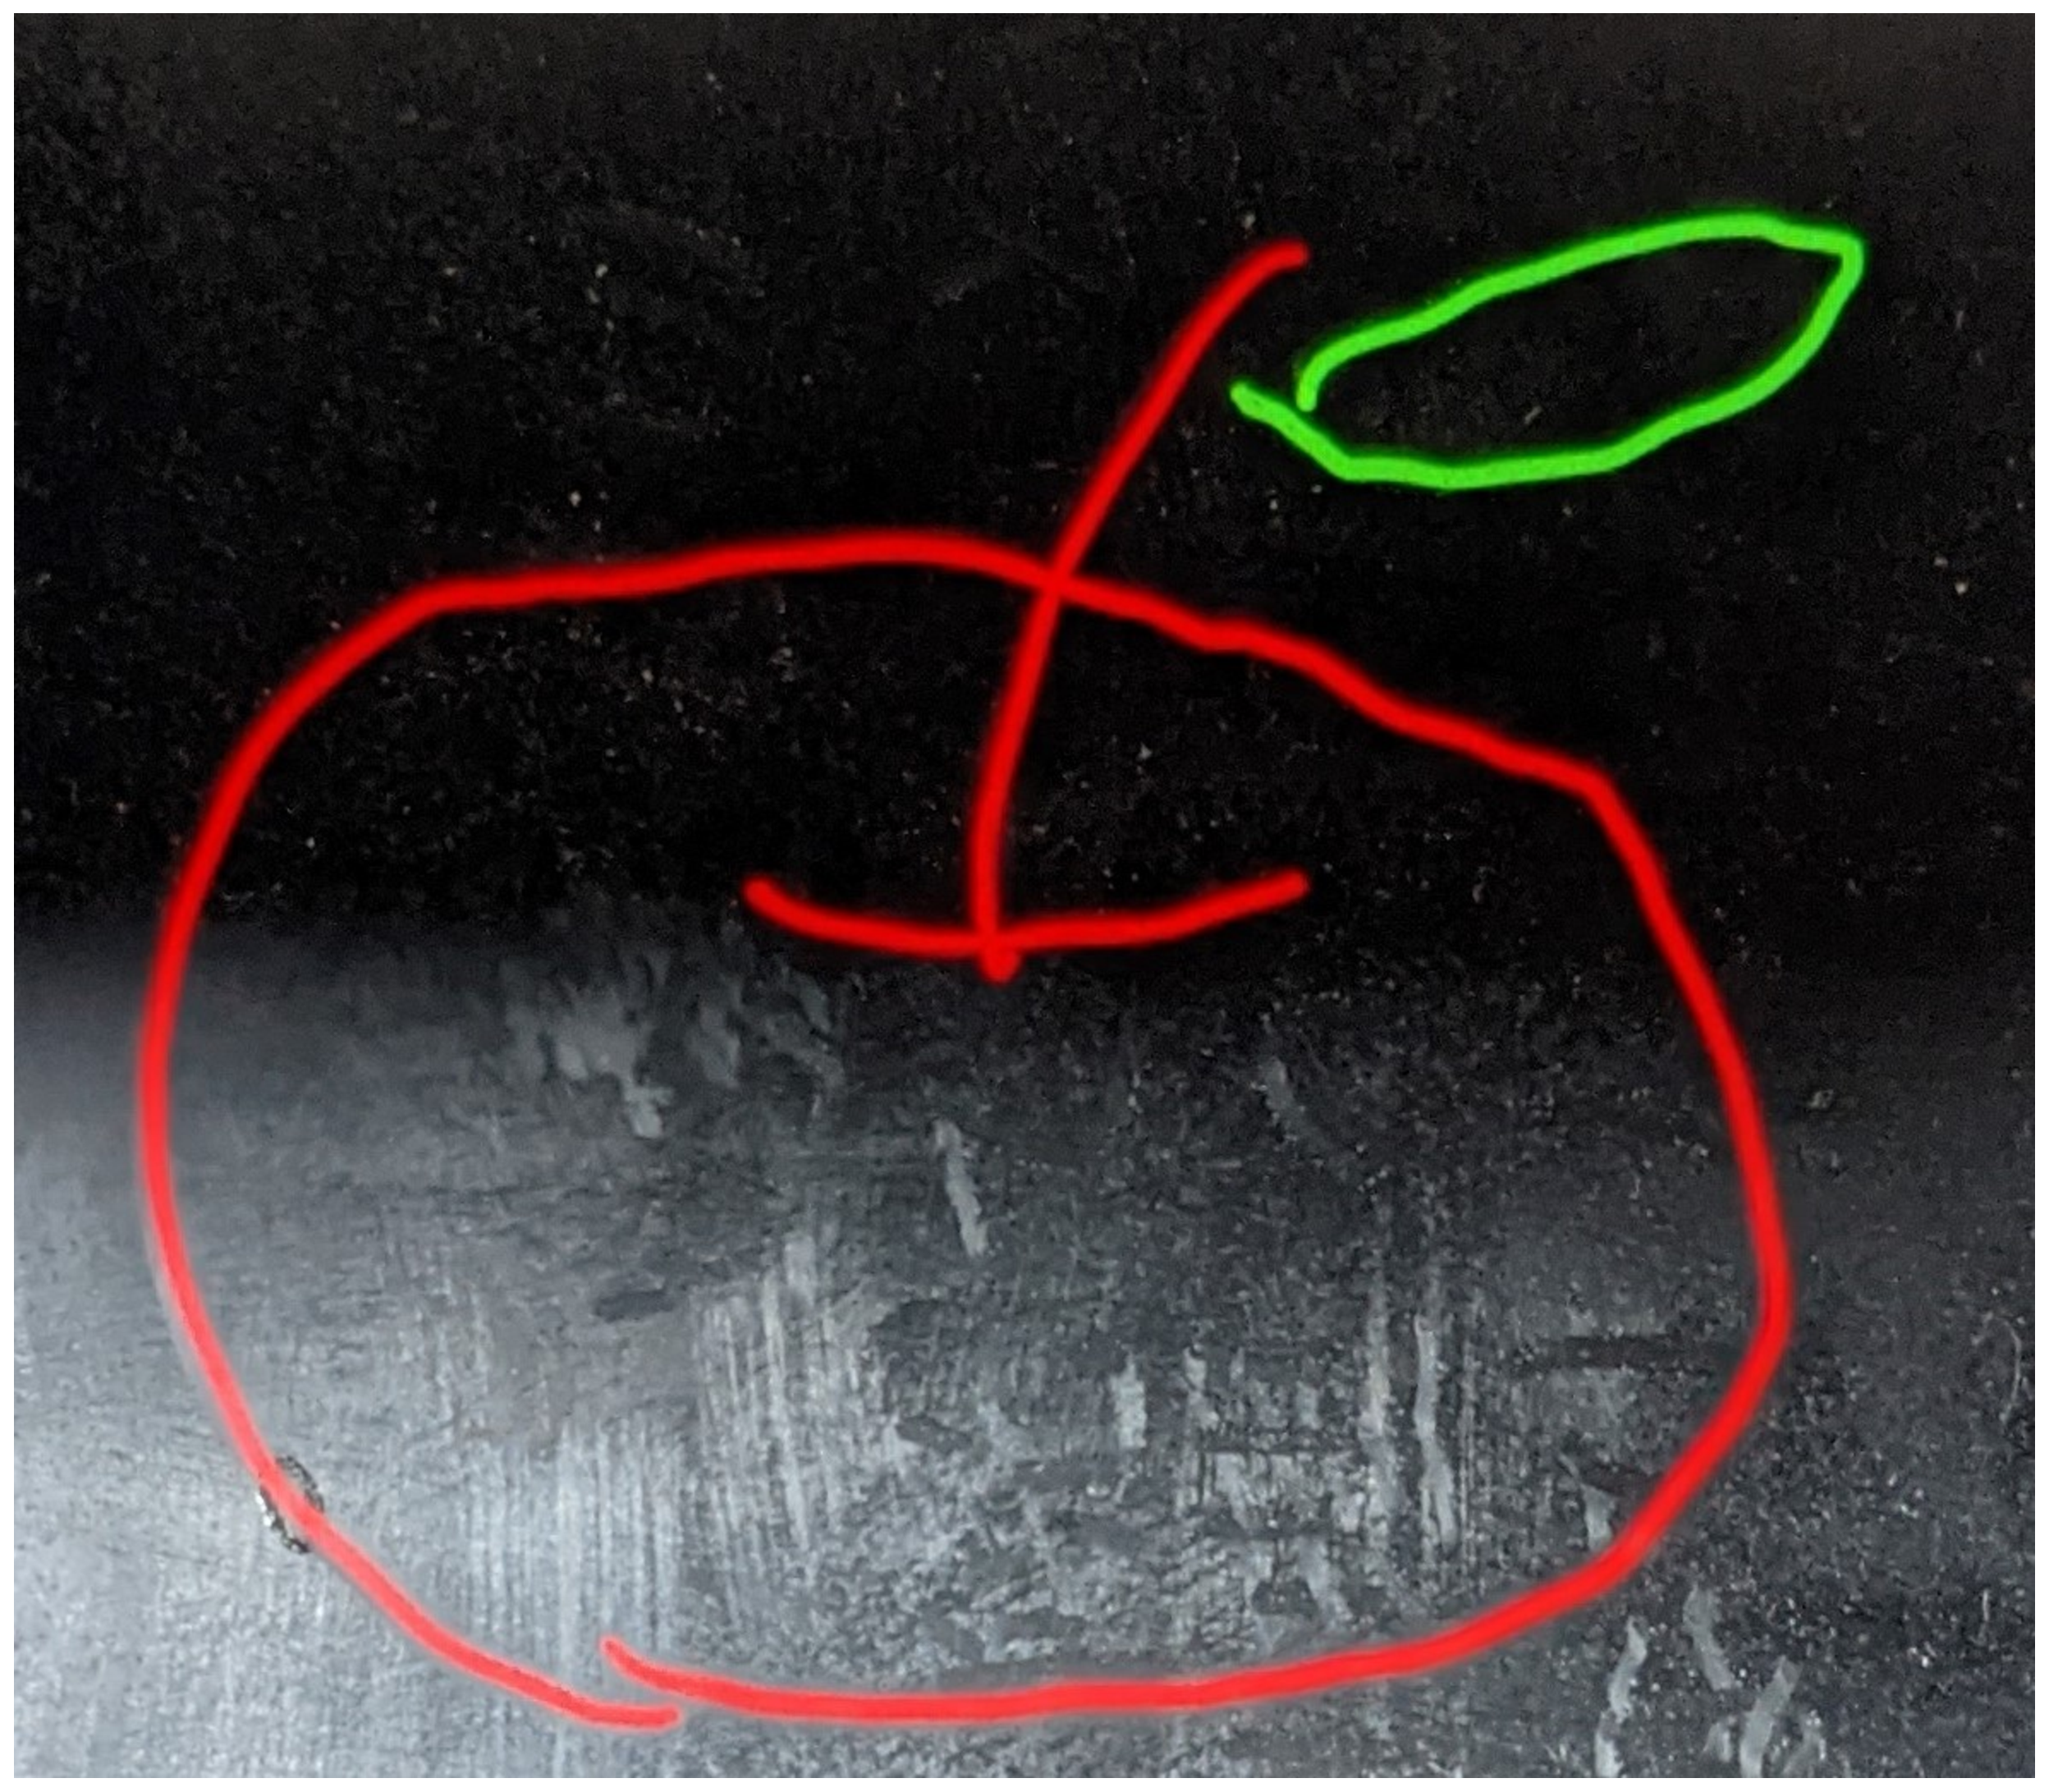
\includegraphics[width=50mm]{apple.eps}
\end{center}
\caption{apple}
\label{fig:apple}
\end{figure}


%
%
\end{document}
